\documentclass[conference]{IEEEtran}
% \IEEEoverridecommandlockouts
% The preceding line is only needed to identify funding in the first footnote. If that is unneeded, please comment it out.
\usepackage{cite}
\usepackage{amsmath,amssymb,amsfonts}
\usepackage{algorithmic}
\usepackage{graphicx}
\graphicspath{{./design/pdf-snapshots/cropped/}}
\usepackage{textcomp}
\usepackage{xcolor}
\usepackage{float}
\usepackage{grffile}
\usepackage{hyperref}
\def\BibTeX{{\rm B\kern-.05em{\sc i\kern-.025em b}\kern-.08em
    T\kern-.1667em\lower.7ex\hbox{E}\kern-.125emX}}
\begin{document}

\title{Correction Techniques for Image Faults}

\author{\IEEEauthorblockN{1\textsuperscript{st} Dominic Gaiero}
\IEEEauthorblockA{\textit{Computer Engineering Department} \\
\textit{California Polytechnic State University, San Luis Obispo}\\
San Luis Obispo, USA \\
dgaiero@calpoly.edu}
\and
\IEEEauthorblockN{2\textsuperscript{nd} Given Name Surname}
\IEEEauthorblockA{\textit{Computer Engineering Department} \\
\textit{California Polytechnic State University, San Luis Obispo}\\
San Luis Obispo, USA \\
email address or ORCID}
}

\maketitle

\begin{abstract}
This document is a model and instructions for \LaTeX.
This and the IEEEtran.cls file define the components of your paper [title, text, heads, etc.]. *CRITICAL: Do Not Use Symbols, Special Characters, Footnotes, 
or Math in Paper Title or Abstract.
\end{abstract}

\begin{IEEEkeywords}
CMOS, CIS
\end{IEEEkeywords}

\section{Introduction}
In this project the effectiveness radiation hardening a device through software was tested.  This expands on past methods by having picture correction happen in the data processing phase, rather than redesigning from a hardware level. While using software to mitigate the effects of radiation on sensors is not a permanent solution, the benefits of significant reduced costs and development make this solution very appealing for less critical applications. This project targets uses in security at a radiation plant or non-critical cameras in space or other radiation intensive conditions. This will allow systems that use cameras in these conditions to operate with more reliability and allow for more clear images despite the conditions and operation of the cameras.  Also, this solution aims to give more information on the nature of a fault in a sensor to a user, unlike traditional image processing techniques.  

\section{CMOS Background}
CMOS(complementary metal oxide semiconductor) sensors are one of the most commonly used modern methods of creating digital images in cameras.  They work by having light filter into a light sensitive diode that is then able to activate a transistor so that a signal can be generated.  (Insert photo of CMOS circuit)  The photo-diode is sensitive to light and is able to generate a current by being exposed to photons.  Finally that signal is sent to a central processor and translated into a pixel.  CMOS sensors are very vulnerable to faults due to radiation and other interferences because in some way the circuit has to be exposed and cannot be fully insulated.  One fault that often occurs in CMOS sensors is a Dark Current.  A Dark Current is when the CMOS circuit is activated by a wave that is not a photon.  In space and other radiation intensive environments this is a very relevant limitation of the technology because extreme accuracy is required with very high consistency.  Radiation that reaches a sensor is likely to cause the sensor to have some kind of fault, and if the intensity of the radiation is high enough then a pixel can become permanently damaged.  These Dark Currents when realized through the circuit and the central processor would appear to be a noisy picture or a collection of white pixels.  These faults can be harmless at first, but given enough time to build up they can render a sensor useless.  
\section{Method}
\subsection{Tools Used}
The model was designed using MATLAB\textsuperscript{\tiny\textregistered} and SIMULINK\textsuperscript{\tiny\textregistered} R2018B. Analysis was also performed using this software. Additionally, to aid testing, a generic video file was used provided by \hyperlink{https://blogs.unity3d.com/2016/11/28/free-vfx-image-sequences-flipbooks/}{Unity3D}.
\subsection{Assumptions}

\begin{figure}[H]
   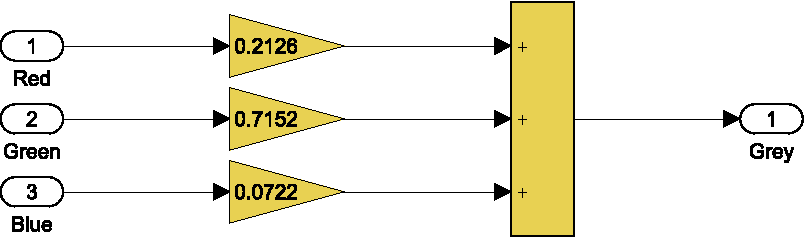
\includegraphics[width=0.5\textwidth]{impl_dsgn_ITU-R BT.709.pdf}
   \caption{System Specifications}\label{fig:sysSpecs}
\end{figure}

\begin{thebibliography}{00}
% http://sirad.pd.infn.it/scuola_legnaro_2009/Presentazioni_Web/18_ScuolaLNL2009_Gerardin_Web.pdf
\bibitem{b1}T. Watanabe, T. Takeuchi, O. Ozawa, H. Komanome, T. Akahori, K. Tsuchiya,  ``A new radiation hardened CMOS image sensor for nuclear plant,''  www.imagesensors.org, 2017.
\bibitem{b2} J. Clerk Maxwell, A Treatise on Electricity and Magnetism, 3rd ed., vol. 2. Oxford: Clarendon, 1892, pp.68--73.
\bibitem{b3} I. S. Jacobs and C. P. Bean, ``Fine particles, thin films and exchange anisotropy,'' in Magnetism, vol. III, G. T. Rado and H. Suhl, Eds. New York: Academic, 1963, pp. 271--350.
\bibitem{b4} K. Elissa, ``Title of paper if known,'' unpublished.
\bibitem{b5} R. Nicole, ``Title of paper with only first word capitalized,'' J. Name Stand. Abbrev., in press.
\bibitem{b6} Y. Yorozu, M. Hirano, K. Oka, and Y. Tagawa, ``Electron spectroscopy studies on magneto-optical media and plastic substrate interface,'' IEEE Transl. J. Magn. Japan, vol. 2, pp. 740--741, August 1987 [Digests 9th Annual Conf. Magnetics Japan, p. 301, 1982].
\bibitem{b7} M. Young, The Technical Writer's Handbook. Mill Valley, CA: University Science, 1989.
\end{thebibliography}

\end{document}